\documentclass{article}

\usepackage[utf8]{inputenc}
\usepackage[pdftex]{graphicx}
\usepackage[left=3cm,right=3cm,top=3cm,bottom=3cm]{geometry}
\usepackage[T1]{fontenc}
\usepackage[francais,english]{babel}
\frenchbsetup{StandardLists=true}
\selectlanguage{english}


\usepackage{amsmath}
\usepackage{amssymb}
\usepackage{mathtools}
\usepackage{slashbox}


\usepackage{caption}
\usepackage[hidelinks]{hyperref}
\usepackage{xcolor}


%ALGORITHM
\usepackage{algorithm}
\usepackage[noend]{algpseudocode}
\renewcommand{\algorithmicforall}{\textbf{for each}}
\newcommand{\var}[1]{\mathit{#1}}
\newcommand{\func}[1]{\mathrm{#1}}
\algdef{SE}[DOWHILE]{Do}{doWhile}{\algorithmicdo}[1]{\algorithmicwhile\ #1}
%

\usepackage{listings}

\usepackage{graphicx}

\renewcommand\thesection{\arabic{section}}

\usepackage{fancyhdr}
\pagestyle{fancy}
\fancyhf{}
\fancyhead[R]{\thepage}


\title{[INFO-F409] Learning Dynamics \\ Second assignment}
\author{\bsc{BUI QUANG PHUONG} Quang Linh \\ Université libre de Bruxelles - ULB ID : 000427796  \\ MA1 Computer Sciences}
\date{December 2018}

\begin{document}

\maketitle

\tableofcontents

\newpage
\section{Part I: Complex networks}

\subsection{1 - Erdos-Renye network}

\subsubsection{Q1 statement}

\textit{Generate Erdos-Renye network (Random networks) [1,2]. Generate the network from scratch and present/describe the part of the code you used to generate the network in your document. For a size of the network of N=10000, calculate a K so that each node has in average degree 4.} 

\subsubsection*{Pseudo-code}

\begin{algorithm}
  \caption{Generation of Erdos-Renye network}\label{euclid}
  \begin{algorithmic}[1]
  \Procedure{ErdosRenye}{$n$, $K$}
  \State Initialize the network edges list
  \ForAll{'future' edges $\equiv 0 \rightarrow K$}:
  \State Pick two random nodes in the network
  \State Define $newEdge$ variable taking the 2 picked nodes  
  \EndFor
  \If {$newEdge$ not already exists}:
  \State Add $newEdge$ in the list of edges
  \EndIf
  \Return list of network's edges  
  \EndProcedure
  \end{algorithmic}
\end{algorithm}

\subsubsection*{Algorithm description} 

The Erdos-Renye network is a random network generated. Before all, we have to initialize a list of edges which will be returned and will form the random network. This edges list is composed by some tuples of 2 elements $(x,y)$ representing the edges where $x,y$ are the two nodes that the edge is connecting. Now, we have to keep creating edges while the number edges $K$ passed in parameters isn't reached. The random part is managed by the step of picking nodes by pair $(x,y)$ in the network which is totally random, all nodes can be picked at this moment. Of course, before accepting the edge between de two nodes chosen, a verification that this edge doesn't already exists, which means that the edge $(x,y)$ \textbf{\underline{and}} $(y,x)$ isn't already created, is done.

\subsection*{K for average degree of 4}

To calculate the value of $K$ for an average degree of 4, first we know that an edge generates a link between two nodes and then increases the degree of two nodes. Moreover, we have 10000 nodes, thus we can calculate the value of $K$ for an average degree of 4 using the following formula : $ \frac{2K}{10000} = 4 $ that gives $K = 20000$. 

\subsubsection{Q2 statement}

\textit{Plot the degree distribution of the generated network. Calculate the mean and standard deviation and plot the normal distribution with these same parameters}

\subsubsection*{Degree distribution} 
The degree distribution of the network generated by the Erdos-Renye algorithm with $K = 20000$ is given by the \autoref{fig:ER-distribution}. 

\begin{figure}[h]
  \centering
  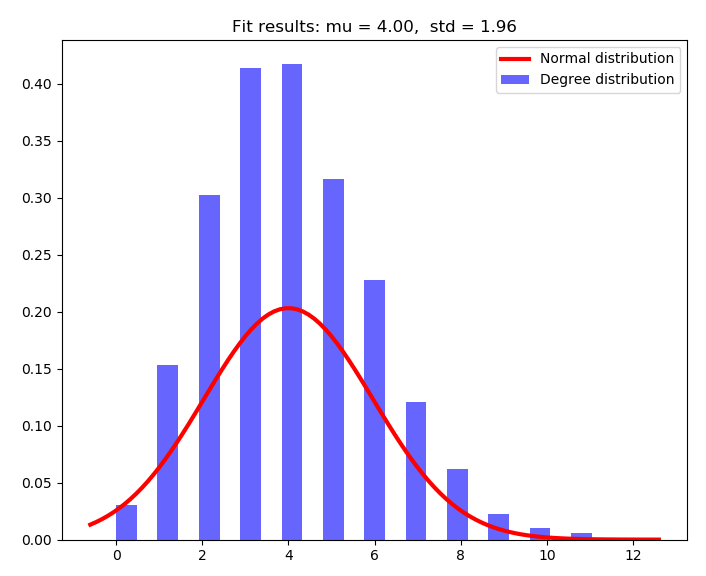
\includegraphics[scale=0.6]{fig/ER-distribution.png}
  \caption{Distribution for Erdos-Renye generated network}
  \label{fig:ER-distribution}
\end{figure}

\subsubsection*{Mean and standard deviation}
The value of the mean in the distribution of \autoref{fig:ER-distribution} is 
$$ \mu = 3.999 $$ and for the standard deviation is $$ \sigma = 1.964 $$. 

\subsection{2 - Barabasi-Albert network}

\subsubsection{Q3 statement}
\textit{Generate a Barabasi-Albert network (Scale Free network) [1,3]. Generate the network from scratch and present/describe the part of the code you used to generate the network in your document.}

\subsubsection*{Pseudo-code} 

\begin{algorithm}
  \caption{Generation of Barabasi-Albert network}\label{euclid}
  \begin{algorithmic}[1]
  \Procedure{BarabasiAlbert}{$Graph$, $N$}
  \State Initialize a fully connected 4 nodes network
  \ForAll{'future' node until $N \equiv 4 \rightarrow N$}:
  \State Add a node $x$ to the network 
  \ForAll{current network's nodes}:
  \State Compute the probability of the added node $x$ being linked to those nodes
  \State Append it into a list $probasLinking$  
  \EndFor
  \State Pick 4 nodes 'randomly' (with their associated probabilities) in the network's nodes
  \For{the 4 picked nodes}:
  \State Link the added node $x$ to them
  \EndFor
  \EndFor
  \State Reinitialize $probasLinking$ and increment by 8 (4 new edges = 8 nodes with their degree increasing by 1) the total degree number for the computation of the next probabilities 
  \EndProcedure
  \end{algorithmic}
\end{algorithm}

\newpage
\subsubsection*{Algorithm description}
The only requirement of the \textit{Barabasi-Albert} algorithm is an initialization of a fully connected 4 nodes network. Now that the graph is initialized, we can start to add nodes one by one until the number $N$ of nodes desired to our network. The number of nodes  $N$ is passed in parameter. At every add, the node $x$ has to be linked to \textbf{\underline{strictly 4}} random nodes (that explains why an initialization of a 4-nodes graph is required). Every node $i$ of the network has a computed probability of being linked to the added node. This computation is done following the formula $$ P_{i} = \frac{k_{i}}{\sum k_{j}} $$ where $k_{i}$ is the degree of the existing node $i$ and $ \sum k_{j}$ is the total degree of the network (sums over all the nodes in the network). The nodes with higher degree have then obviously more chance to be linked to the added node $x$. The pick phase is then not totally random.  Once the 4 nodes are chosen, we simply add an edge between the 4 picked nodes and the added node $x$. Finally, reinitialize the probabilities and increment the total degree number by 8 for the next probabilities computation. Repeat it until $N$ nodes are added. 


\subsubsection{Q4 statement}
\textit{Plot the degree distribution of the generated network using a linear scale on both axes. Plot in the same figure an exponential distribution which looks similar and reports on the parameters of that distribution.}

\subsubsection*{Degree distribution and exponential distribution} 
The degree distribution of the network generated by the Barabasi-Albert algorithm with $N = 10000$ is given by the \autoref{fig:BA-distribution}. Note that it exists some nodes with degree more than 100, but actually not visible in the \autoref{fig:BA-distribution} because the counter for those degrees are too small. Thus, a zoom of this interval is presented in the \autoref{fig:BA-distribution-zoom}. Moreover, the exponential distribution which looks similar is plotted in the figures in red. Concerning the parameters of that distribution, an exponential function is then used to fit the degree distribution. This exponential function follows the probability density function formula of this kind of distribution : $$\lambda e^{\lambda x}$$ that gives : $$a*exp(-b*x)+c$$ where $x$ is the degree distribution and $a,b,c$ arbitrary values.   
% REPORT PARAMETERS 

\begin{figure}[h]
  \centering
  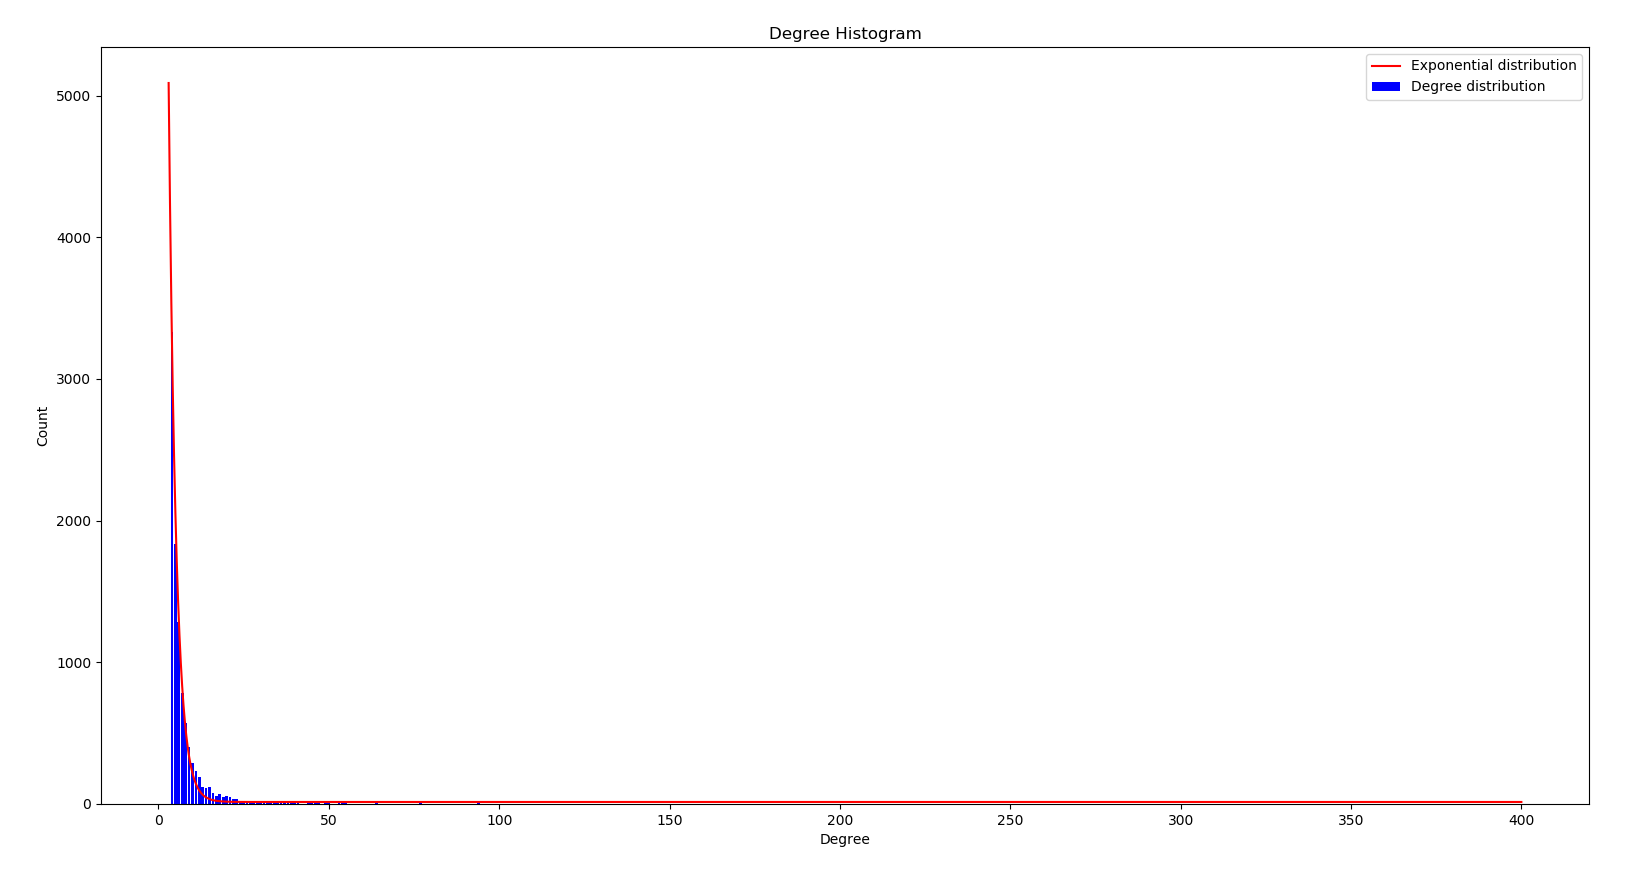
\includegraphics[scale=0.35]{fig/BA-distribution.png}
  \caption{Distribution for Barabasi-Albert generated network}
  \label{fig:BA-distribution}
\end{figure} 

\newpage
\begin{figure}[h]
  \centering
  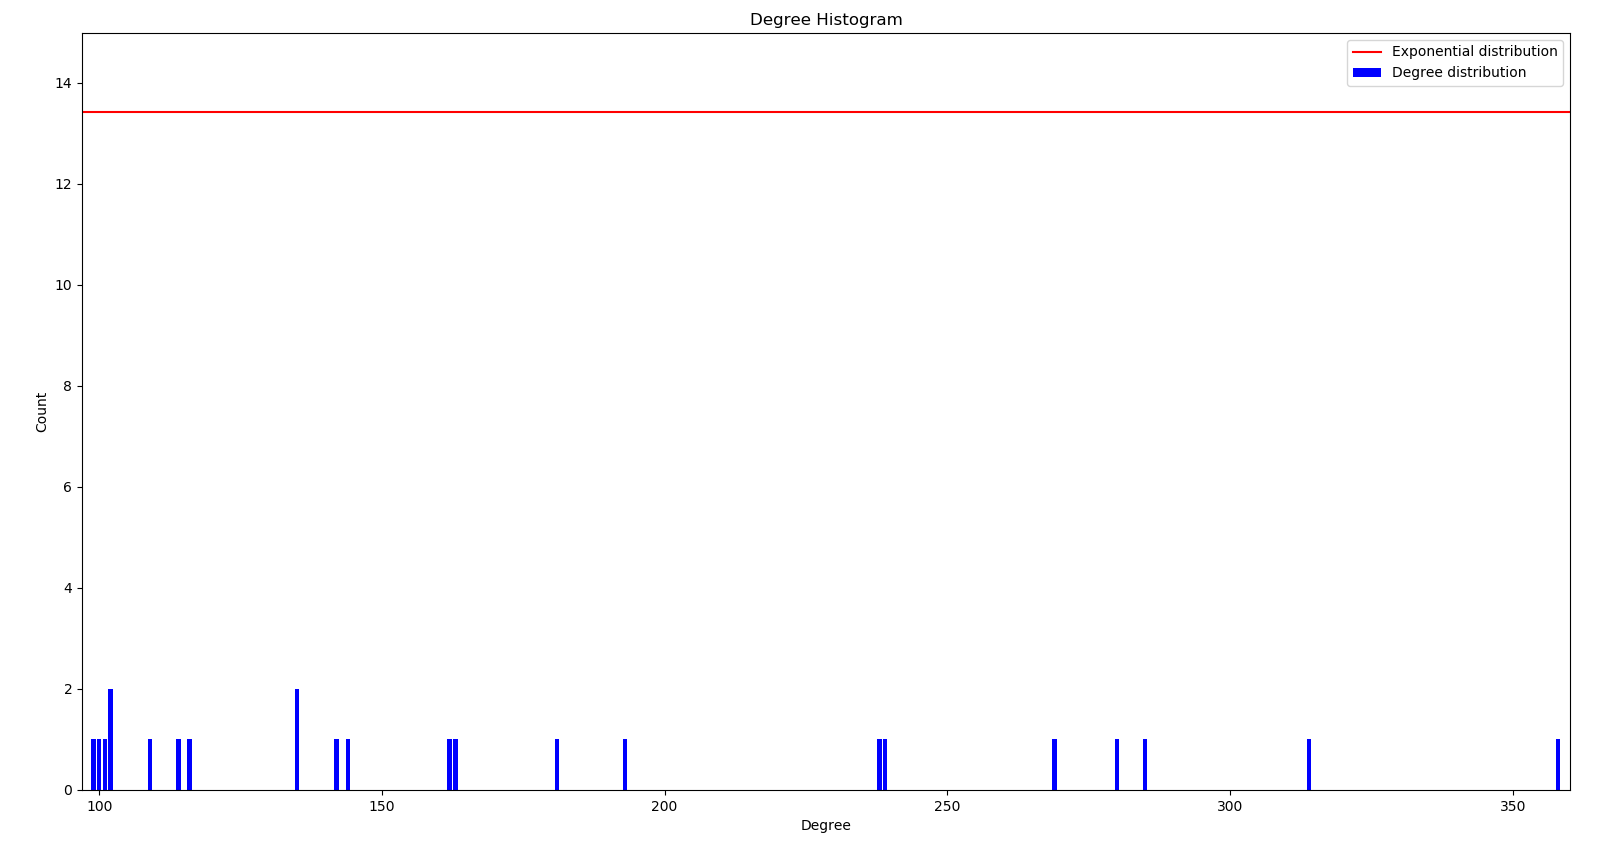
\includegraphics[scale=0.3]{fig/BA-distribution-zoom.png}
  \caption{Zoom of the interval 100-400 in the BA generated network distribution}
  \label{fig:BA-distribution-zoom}
\end{figure} 


\subsubsection{Q5 statement}
\textit{Plot the same distribution on log-log scale. Fit the distribution using Least Square fit. You can use existing functions for fitting and plot the fit next to the data. What are the parameters of the fit? How does it fit? Why? Write a paragraph about why we should not use Least Square fit to fit power laws.}

\subsubsection*{Distribution on log-log scale} 
The same degree distribution of the network generated by the Barabasi-Albert presented in \autoref{fig:BA-distribution} in log-log scale is shown in the \autoref{fig:BA-distribution-log}. 

\begin{figure}[h]
  \centering
  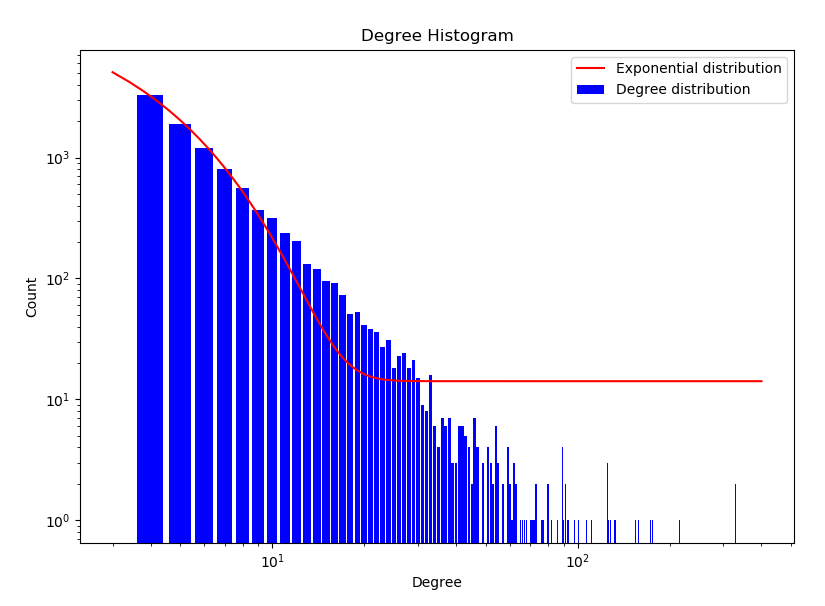
\includegraphics[scale=0.55]{fig/BA-distribution-log.png}
  \caption{Distribution for Barabasi-Albert generated network in log-log scale}
  \label{fig:BA-distribution-log}
\end{figure}

\subsubsection*{Fitting using Least Square Fit} 

The fitting on the log-log scale distribution using Least Square Fit is presented in \autoref{fig:BA-LSF}. The parameters used are simply a fit function and an error function. The fit function is creating the fit line following a linear model to approximate the data set $(x,y)$ where $x$ is the network's degree list and $y$ the corresponding counters of degrees $x$ (i.e. degree $x_{i}$ is counted $y_{i}$ times in the network). The least square fit function is trying to minimize the sum of the squares of the residuals (difference between real data and fitted data). The fit function is then of the form : $$ y = a \cdot x^{b} $$. The error function is calculating the "error bar" (for this fitting, we arbitrary chose an error rate of 10\%) for each point of the distribution.  \\

The fit is not going well, most of the error bars (or even the points) of the distribution points are missing the fit line. 

% EXPLIQUER POURQUOI 

\begin{figure}[h]
  \centering
  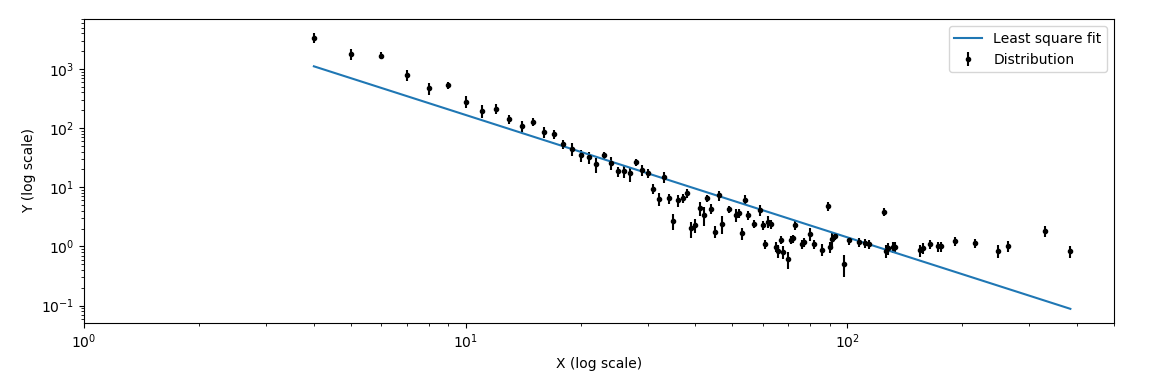
\includegraphics[scale=0.5]{fig/BA-LSF.png}
  \caption{Least Square Fit on log-log scale BA distribution}
  \label{fig:BA-LSF}
\end{figure} 


\subsubsection{Q6 statement}
\textit{Plot cumulative distribution and fit it with Least Square Fit, report the obtained parameters and plot of the fitted function.}

\subsubsection*{Plotting result and parameters} 
The cumulative distribution of the Barabasi-Albert network is given by the \autoref{fig:BA-Cumulative}. The distribution is plotted in lin-lin scale. 

% FIT AND PLOT PARAMETERS + FITTED FUNCTION

\begin{figure}[h]
  \centering
  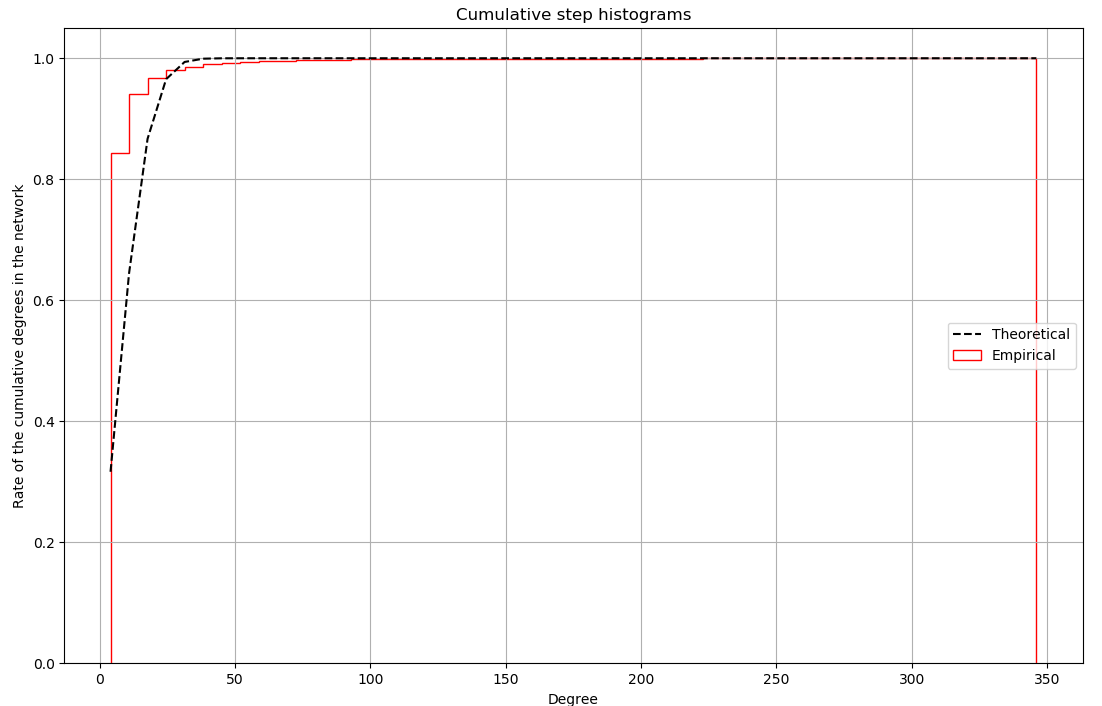
\includegraphics[scale=0.4]{fig/BA-Cumulative.png}
  \caption{Cumulative distribution of BA network}
  \label{fig:BA-Cumulative}
\end{figure}


\subsubsection{Q7 statement}
\textit{Now fit your distribution using maximum likelihood method. You can use any of the packages which has the method developed.}


\subsubsection{Q8 statement}
\textit{Report the parameters of the fit and plot them next to distribution.}

\subsubsection{Q9 statement}
\textit{Compare the power law fit with the exponential fit (using the same package). Report the log likelihood ratio R and the p-value. What do these numbers mean?}


\subsubsection{Q10 statement}
\textit{What is the mathematical formula for scale free distribution you generated? Calculate the mean and the standard deviation of function? What would be the mean and standard deviation if the exponent would be 2.5?}

\newpage 
\section{Part II: Game Theory on Networks}

\subsection{Question 1 - Prisoner's dilemma on networks}

\subsubsection*{Statement}
\textit{Run a simulation of agents playing Prisoner's Dilemma on the generated networks. Explain why would we set up the probability $P_{ij}$ like this? Why does it make sense to update your actions like that?} 

\subsubsection{Description of the problem}
In this part of the assignment, we are trying to play the prisoner's dilemma game on the previous networks generated by the Erdos-Renye and Barabasi-Albert algorithms. As a reminder, the prisoner's dilemma is a game in which two players each have two options : "Cooperate" or "Defect" whose payoffs depends on the simultaneous choice made by the other. In this section, we will simulate each node of the network as an agent playing the game with every of its neighbours. The payoff of a node is calculated by the sum of all the payoffs gained for each of its neighbours. To summarize the procedure of the game on our networks : 
\begin{enumerate}
\item First round: each node randomly pick "Cooperate" or "Defect" 
\item Rest of rounds: every node $i$
\begin{enumerate}
\item picks randomly one of its neighbour $j$
\item adapts the strategy chosen related to the action of $j$ by copying the action of $j$  with a certain probability $$ P_{ij} = \frac{W_{j}-W_{i}}{k_{max} D_{max}} $$ where $W_{i}$, $W_{j}$ are respectively the total payoff of the current node $i$ and of the picked neighbour $j$, $k_{max}$ the maximum degree between nodes $i$ and $j$, $D_{max} = max(T,R) - min(S,P)$ corresponding to the gap between the best possible payoff and the worst possible payoff.  
\end{enumerate} 
\end{enumerate}  

In our case, the matrix showing the payoff for each combination of actions between node 1 and 2 is given in the \autoref{fig:payoff-IPD}.
 
\begin{figure}[h]
  \centering
  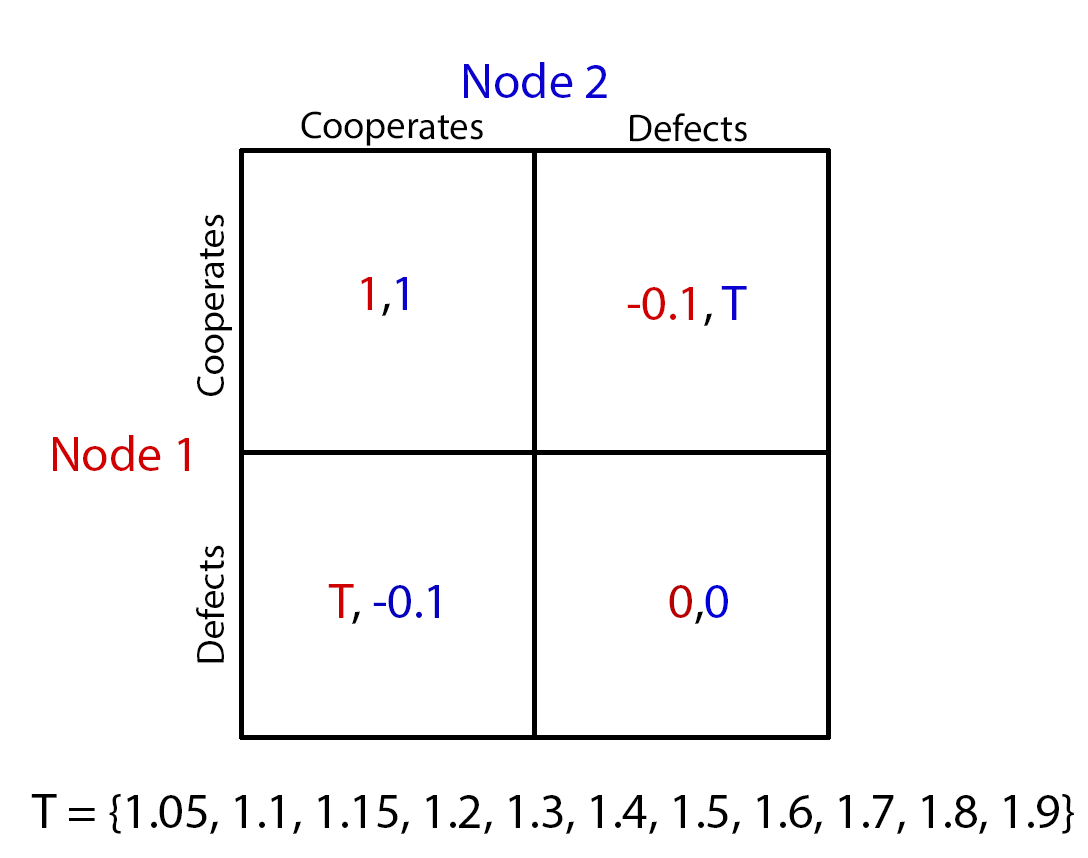
\includegraphics[scale=0.9]{fig/payoff-IPD.png}
  \caption{Payoffs matrix for the prisoner's dilemma game}
  \label{fig:payoff-IPD}
\end{figure}

\subsubsection{Adapting the strategy}
The question is now why does it make sense for a node to adapt its strategy by following the probability $P_{ij}$ ? Let's analyse the formula step by step : 

\begin{itemize}
\item In the numerator we find $W_{j} - W_{i}$, corresponding to the difference between the payoff of the neighbour $j$ and the payoff of the node $i$ itself. That means that more the payoff of $W_{j}$ is high, more the numerator will be high, then more the probability will have a huge value. It makes obviously a sense. More the payoff of the neighbour $j$ is high, more the node $i$ will try to copy the strategy of $j$ to get a higher payoff. 
\item Concerning the denominator, we find the product between $k_{max}$ and $D_{max}$ which are then inversely proportional to the probability $P_{ij}$. First, $k_{max}$ is the highest degree between $i$ and $j$, it means that if $j$ has a higher degree, he will have more chance to have a higher payoff because of summing more payoffs \textbf{even if he sums bad strategies payoffs}. Thereby, the fact that a payoff is higher is not necessarily due to a good strategy choice but can be due by summing a high number of payoff. In this case, more huge is the degree of $j$, less adapting the strategy of $i$ is a good choice. Dividing the numerator by $k_{max}$ is then necessary to decreases the chance to copy a bad strategy and then creating a good balance with the numerator.  
Moreover, concerning $D_{max}$, more the gap between the best the best strategy payoff and the worst one is big, more the payoff of the bad strategy is big. Thus, it is more critical to adapt the worst strategy. This $D_{max}$ is then useful for a question of safety which means that the node $i$ prefers to not gain more instead of losing a lot. Indeed, more $D_{max}$ is high, more the bad strategy has a huge impact, less the node $i$ will risk to change to maybe adopts a worse strategy.  
\end{itemize}

\subsection{Question 2 - Stationary state of cooperation level}

\subsubsection*{Statement}
\textit{Plot the cooperation level over time for all the values of T and for both networks. Establish after how many rounds the system reaches stationary state (when the level of cooperation does not change too much).}

\subsubsection{Plot result}
The following plotting outcomes are got by simulating the prisoner's dilemma game on 1000 rounds. We arbitrary chose to pick a huge number of rounds to have more accuracy in the result. The \autoref{fig:IPD-ER} presents the plot of the simulation on the network generated by Erdos-Renye algorithm while the \autoref{fig:IPD-BA} presents the simulation on the network generated by Barabasi-Albert algorithm. 


\begin{figure}[h]
  \centering
  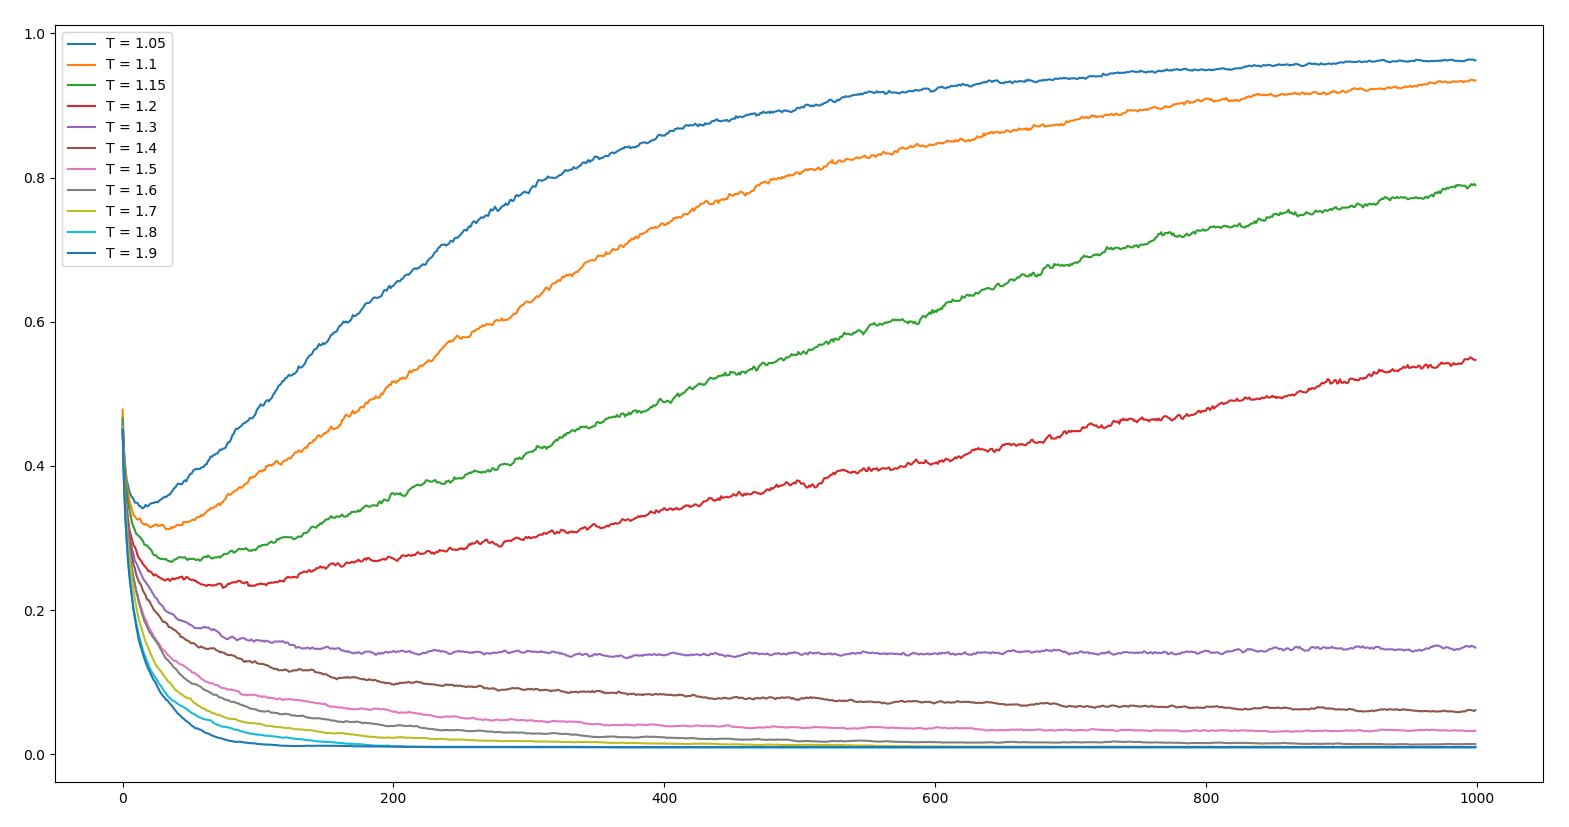
\includegraphics[scale=0.32]{fig/ER-1000rounds.png}
  \caption{Cooperation rate for prisoner's dilemma game on \textbf{Erdos-Renye} network for 1000 rounds}
  \label{fig:IPD-ER}
\end{figure}

\newpage
\begin{figure}[h]
  \centering
  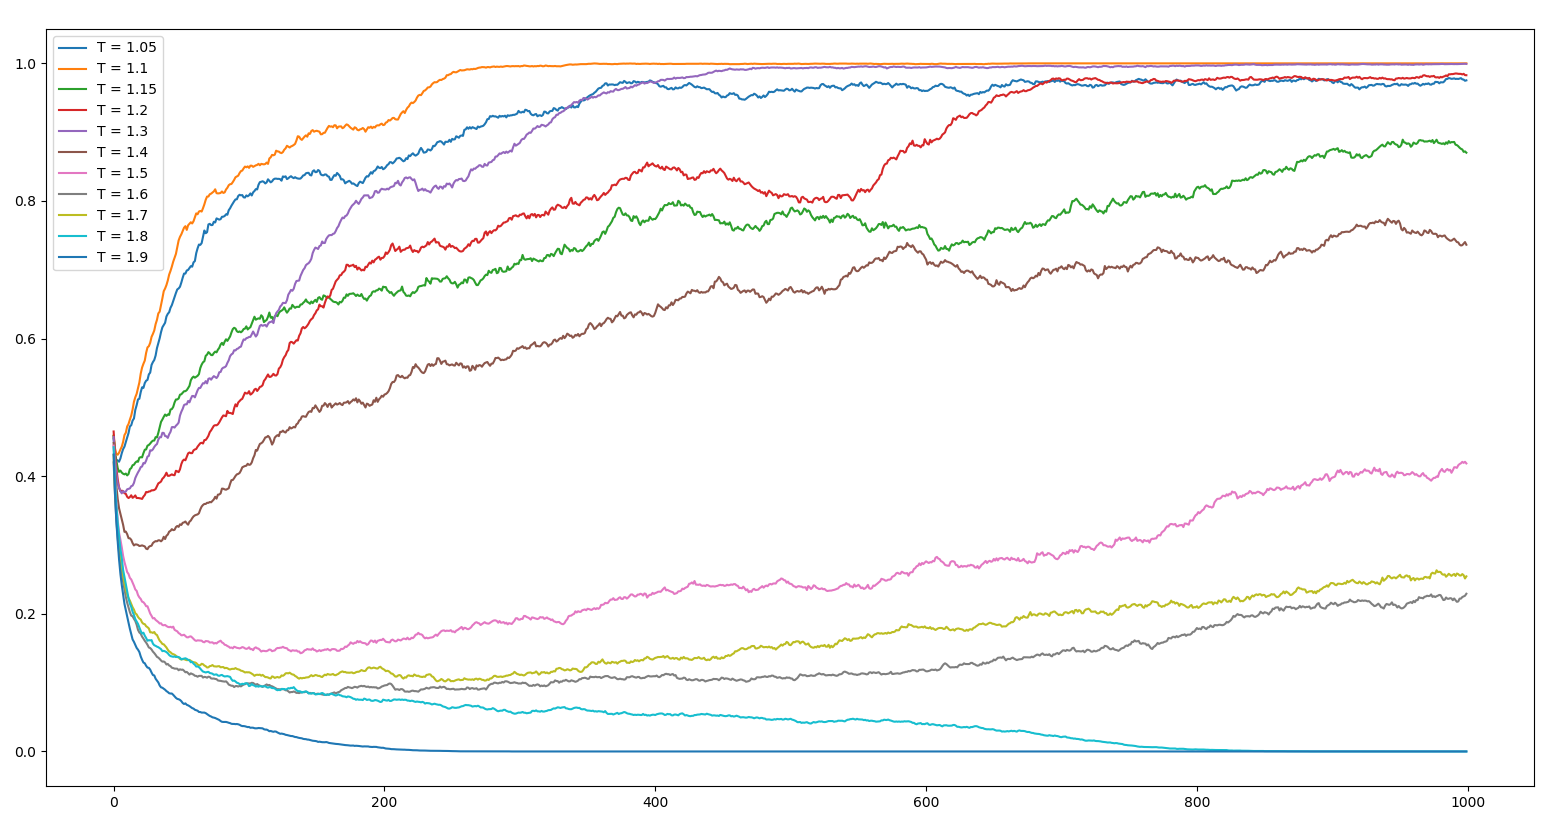
\includegraphics[scale=0.32]{fig/BA-1000rounds.png}
  \caption{Cooperation rate for prisoner's dilemma game on \textbf{Barabasi-Albert} network for 1000 rounds}
  \label{fig:IPD-BA}
\end{figure}

\subsubsection{Stationary state}
\textbf{For Erdos-Renye :} Generally, in the case of a graph generated randomly, we observe that more the value of $T$ is small, more quickly the cooperation rate will converge to 1.  We can distinct 2 "sides" of $T$ value. For all the $T \le 1.2$ (i.e. the top side), the cooperation rate will increase and converges to 1 while from a value of $T \ge 1.3$ (i.e. the bottom side), the cooperation rate will converge or stay steady in a value near to 0. For this generated graph, the stationary state depends of the value of $T$. For the bottom side (i.e. $T \ge 1.3$), the stationary state seems to be near 100-150 rounds. On the other side, for $T \le 1.2$, the stationary state approaches more near 450-500 rounds. \\

\noindent
\textbf{For Barabasi-Albert :} Concerning the scale-free network, the cooperation rate is not really steady, we observe a lot of variations so that we can note the cooperation rate decreasing just after being increased and vice versa. The difference that could make this variation is the fact that in a scale-free network, it can exists a node with a high degree (i.e. more than 200-300 for a 10000 nodes network). As a node adapts his strategy according to his neighbour, in such a case, all the nodes connected to the 'high degree' node are potentially changing then creating a variation in the curve. Nevertheless, the general behaviour of the cooperation level over time is quite the same than for random networks. For a value of $T \le 1.4$, the curves seems to converge to one while for a $T \ge 1.5$, the curves are more converging to 0. Thus, as the random graph, the stationary state depends of the value of $T$. For the bottom side (i.e. $T \ge 1.5$), the stationary state seems to be near 200-300 rounds. On the other side, for $T \le 1.4$, the stationary state appears more near 800 rounds.  

\subsection{Question 3 - Average of the stationary cooperation}

\subsubsection*{Statement}
\textit{Average the stationary cooperation level over 100 simulations (for each T and both networks). Plot the dependence of the stationary cooperation level on the value of T for both networks.}

\subsubsection{Plot result}

\begin{figure}[h]
  \centering
  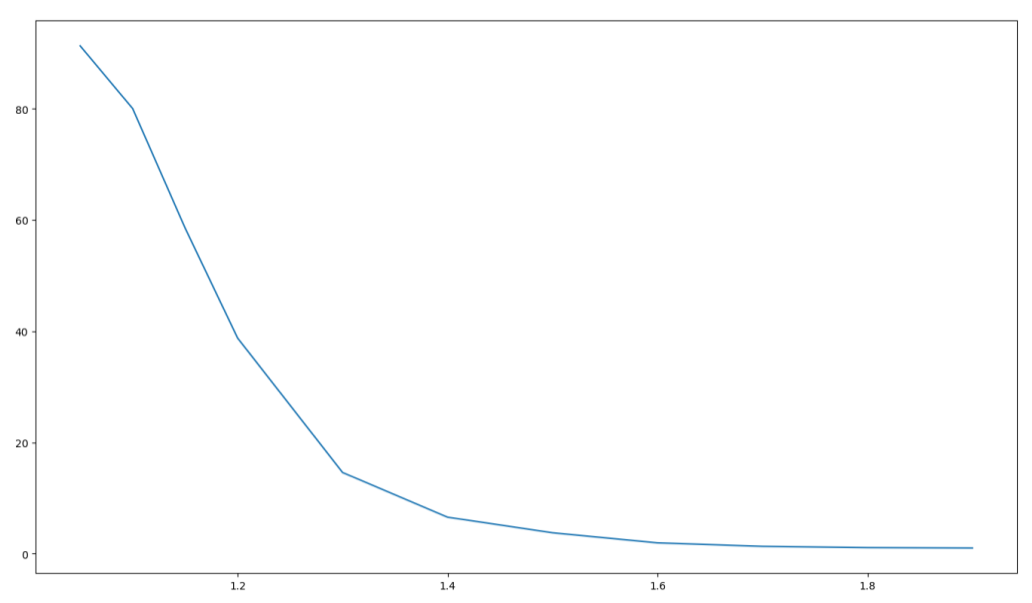
\includegraphics[scale=0.32]{fig/ER-stationary-10sim.png}
  \caption{Average of stationary cooperation level on 100 simulations for \textbf{Erdos-Renyi} network}
  \label{fig:IPD-ER-average}
\end{figure}

\begin{figure}[h]
  \centering
  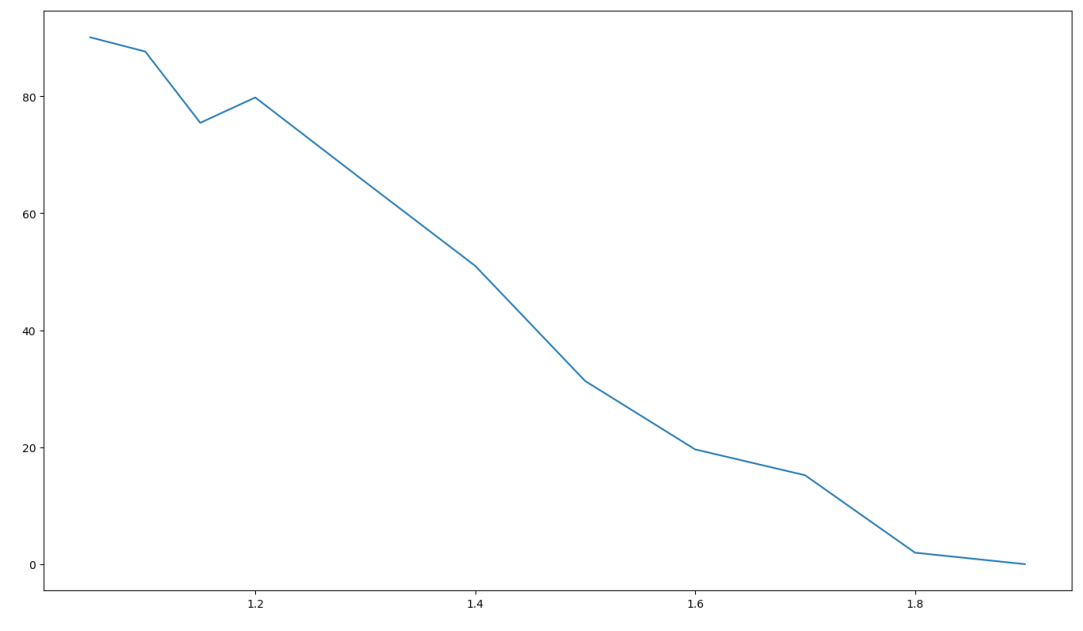
\includegraphics[scale=0.32]{fig/BA-stationary-10sim.png}
  \caption{Average of stationary cooperation level on 100 simulations for \textbf{Barabasi-Albert} network}
  \label{fig:IPD-BA-average}
\end{figure}

\subsection{Question 4 - Difference between the cooperation levels}

\subsubsection*{Statement}
\textit{Comment the differences of the final cooperation levels.}

\subsubsection{Result}

\end{document}